\tableofcontents

\newpage

\section{Задание}
По выданному преподавателем варианту восстановить текст заданного варианта программы и подпрограммы (программного комплекса), определить предназначение и составить его описание, определить область представления и область допустимых значений исходных данных и результата, выполнить трассировку программного комплекса.

\begin{figure}[H]
\centering
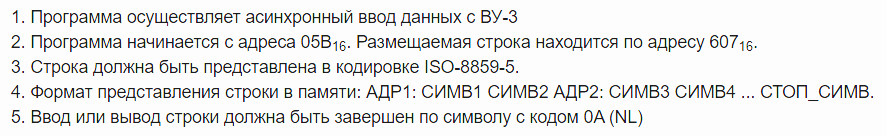
\includegraphics[scale=0.6]{task}
\label{pic:task}
\end{figure}


\section{Текст программы}
\subsection{Основная программа}
\begin{flushleft}
		\begin{tabular}{|c|c|c|l|}
			\hline
			\multicolumn{1}{|c}{\makecell{\textbf{Адрес}\\\textbf{ячейки}}}
			&\multicolumn{1}{|c|}{\makecell{\textbf{Содержимое}\\\textbf{ячейки}}}
			&\multicolumn{1}{|c|}{\makecell{\textbf{Мнемоника}}}
			&\multicolumn{1}{c|}{\makecell{\textbf{Комментарии}}}\\
			\hline
			39C & 0200 & CLA & Очистка аккумулятора \\

			39D & EE19 & ST IP + 25 & Сохраненине 0 в ячейку 0x3B7 \\
			\hline
			39E & AE16 & LD IP + 22 & Загрузка в AC содержимого из ячейки 0x3B5 \\

			39F & 0C00 & PUSH & Запись AC в стек \\

			3A0 & D6FF & CALL 6FF & Вызов подпрограммы по адресу 0x6FF \\

			3A1 & 0800 & POP & Чтение из стека в AC \\

			3A2 & 6E14 & SUB IP + 20 & Вычитание из AC содержимого ячейки 0x3B7 \\

			3A3 & EE13 & ST IP + 19 & Сохраненине AC в ячейку 0x3B7 \\

			\hline
			3A4 & AE0F & ST IP + 15 & Загрузка в AC содержимого из ячейки 0x3B4 \\

			3A5 & 0740 & DEC & Декремент AC\\

			3A6 & 0C00 & PUSH & Запись AC в стек\\

			3A7 & D6FF & CALL 6FF & Вызов подпрограммы по адресу 0x6FF\\

			3A8 & 0800 & POP & Чтение из стека в AC\\

			3A9 & 4E0D & ADD IP + 13 & Сложение AC с содержимым ячейки 0x3B7 \\

			3AA & EE0C & ST IP + 12 & Сохраненине AC в ячейку 0x3B7 \\
			\hline
			3AB & AE0A & LD IP + 10 & Загрузка в AC содержимого ячейки 0x3B6 \\

			3AC & 0700 & INC & Инкремент AC \\

			3AD & 0C00 & PUSH & Запись AC в стек \\

			3AE & D6FF & CALL 6FF & Вызов подпрограммы по адресу 0x6FF\\
			3AF & 0800 & POP & Чтение из стека в AC \\

			3B0 & 0740 & DEC & Декремент AC \\

			3B1 & 4E05 & ADD IP + 5 & Сложение AC с содержимым ячейки 0x3B7 \\

			3B2 & EE04 & ST IP + 4 & Сохранение AC в ячейку 0x3B7 \\

			3B3 & 0100 & HLT & Остановка ТГ \\
			\hline
			3B4 & ZZZZ & Z & Переменная \\

			3B5 & YYYY & Y & Переменная \\

			3B6 & XXXX & X & Переменная \\

			3B7 & 0D08 & R & Результат \\
			\hline
	\end{tabular}
\end{flushleft}

\newpage




\subsection{Подпрограмма}
\begin{flushleft}
	\begin{tabular}{|c|c|c|l|}
		\hline
		\multicolumn{1}{|c}{\makecell{\textbf{Адрес}\\\textbf{ячейки}}}
		&\multicolumn{1}{|c|}{\makecell{\textbf{Содержимое}\\\textbf{ячейки}}}
		&\multicolumn{1}{|c|}{\makecell{\textbf{Мнемоника}}}
		&\multicolumn{1}{c|}{\makecell{\textbf{Комментарии}}}\\
		\hline
		6FF & AC01 & LD \&1 & Чтение из стека входного параметра \\

		700 & F207 & BMI IP + 7 & Если значение параметра меньше нуля, то\\ & & & переход в ячейку 0x708 \\
		701 & 7E09 & CMP IP + 9 & Сравнение AC с содержимым ячейки 0x70B \\

		702 & F905 & BGE IP + 5 & Если значение параметра больше или равно, то\\ & & & переход в ячейку 0x708 \\

		703 & 0500 & ASL & Арифметический сдвиг влево \\

		704 & 0500 & ASL & Арифметический сдвиг влево \\

		705 & 4C01 & ADD \&1 & Сложение входного параметра с AC \\

		706 & 4E05 & ADD IP + 5 & Сложение сожержимого ячейки 0x70C с AC \\
		707 & CE01 & BR IP + 1 & Безусловный переход в ячейку 0x709 \\

		708 & AE02 & LD IP + 2 & Загрузка в AC содержимого ячейки 0x70B\\
		709 & EC01 & ST \&1 & Сохранение AC на место входного параметра в стеке \\
		70A & 0A00 & RET & Возврат из подпрограммы \\
		\hline
		70B & 0B10 & a & Локальная переменная \\

		70C & 00FA & b & Локальная переменная \\
		\hline	
	\end{tabular}
\end{flushleft}

\section{Описание программы}
\subsection{Назначение программы и реализуемая ею функция}
\subsubsection{Реализуемая программой функция}
	\begin{center}
		$ R = F(Y)+F(Z-1)+F(X+1)-1 $
	\end{center}
\subsubsection{Реализуемая подпрограммой функция}
	\begin{center}
		\[
			F(x) =  \begin{cases}
			2832 & \textrm{, для } x < 0\textrm{,}\\
			5x + 250 & \textrm{, для } 0 \leq x < 2832\textrm{,}\\
			2832 & \textrm{, для } x \geq 2832\textrm{,}\\
			\end{cases}
		\]
	\end{center}

\subsubsection{График функции, реализуемый подпрограммой}
\begin{figure}[H]
	\centering
	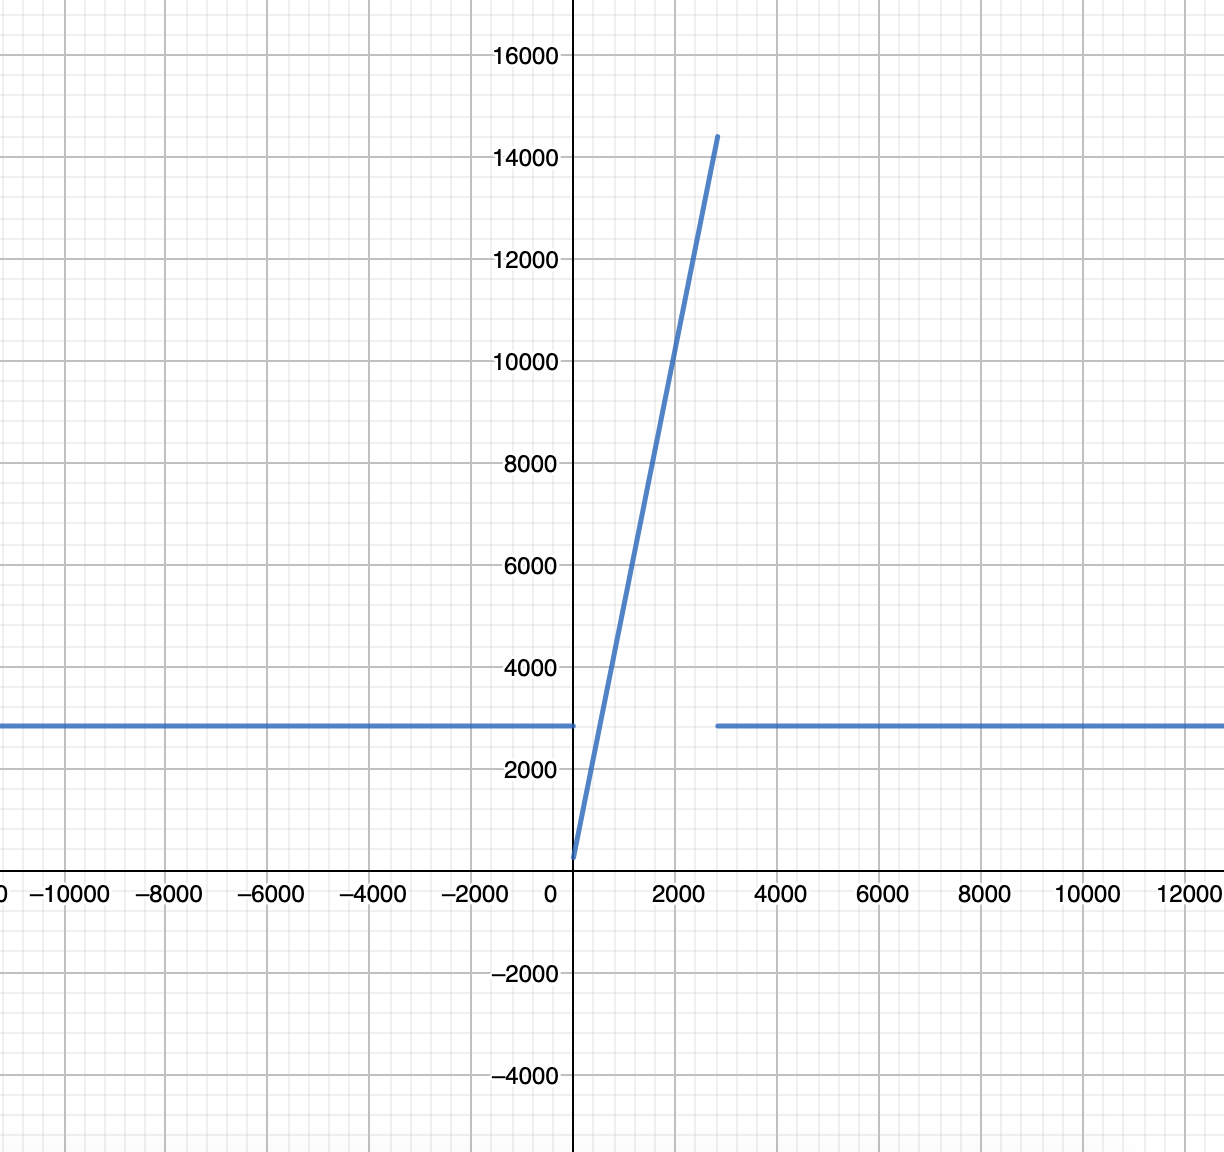
\includegraphics[scale=0.5]{graph}
	\label{pic:graph}
\end{figure}

\subsection{Область представления и область допустимых значений исходных данных и результата}
\subsubsection{Область представления}
\noindent Z, Y, X, R: 16-разрядные знаковые числа с фиксированной запятой. Диапазон значений формата: $-2^{15}\ldots2^{15}-1$

\subsubsection{Область допустимых значений}
\noindent Область допустимых значений R: $749\ldots32764$\\
Пусть $ F(x) $ - реализуемая подпрограммой функция, тогда ОДЗ для нее будет $250\ldots14405$.\\
\\
Входные аргументы (все условия должны выполняться одновременно):\\
Область допустимых значений входного аргумента $ X $: $ -32769...32766 $\\
Область допустимых значений входного аргумента $ Y $: $ -32768...32767 $\\
Область допустимых значений входного аргумента $ Z $: $ -32767...32768 $\\
\\
Если $-1 \leq X < 2831$ и $0 \leq Y < 2832 $ и $1 \leq Z < 2833$, то:\\
\noindent ОДЗ для $ X $: $ -1...6403-Y-Z $.\\
\noindent ОДЗ для $ Y $: $ 0...6403-X-Z $.\\
\noindent ОДЗ для $ Z $: $ 1...6403-Y-X $.\\

\subsection{Расположение в памяти ЭВМ программы, исходных данных и результатов}
\subsubsection{Исходные данные и результат}
\noindent Z (0x3B4) - первый аргумент\\
Y (0x3B5) - второй аргумент\\
X (0x3B6) - третий аргумент\\
R (0x3B7) - результат выполнения программы

\subsubsection{Программа}
\noindent 0x39C --- 0x3B3 - основная программа\\
0x6FF --- 0x70A - подпрограмма\\
a (0x70B), b (0x70C) - локальные переменные, используемые подпрограммой

\subsection{Адреса первой и последней выполняемой команд программы}
\noindent 0x39C - первая исполняемая команда программы\\
0x3B3 - последняя исполняемая команда программы

\newpage
\section{Таблица трассировки}

% \noindent Z = -16162 = 40DE\\
% Y = 24780 = 60CC\\
% X = 1539 = 603\\

\begin{flushleft}
	\begin{tabular}{|c|c|c|c|c|c|c|c|c|c|c|c|c|}
		\hline
		\multicolumn{2}{|c|}{\makecell{\textbf{Выполняемая}\\\textbf{команда}}}
		&\multicolumn{9}{c|}{\textbf{Содердимое регистров после выполнения команды}}
		&\multicolumn{2}{c|}{\makecell{\textbf{Ячейка,}\\\textbf{содержимое}\\\textbf{которой}\\\textbf{ изменилось}}}\\
		\hline
		\multicolumn{1}{|c|}{\makecell{\textbf{Адрес}}}
		&\multicolumn{1}{c|}{\makecell{\textbf{Код}}}
		&\multicolumn{1}{c|}{\makecell{\textbf{IP}}}
		&\multicolumn{1}{c|}{\makecell{\textbf{CR}}}
		&\multicolumn{1}{c|}{\makecell{\textbf{AR}}}
		&\multicolumn{1}{c|}{\makecell{\textbf{DR}}}
		&\multicolumn{1}{c|}{\makecell{\textbf{SP}}}
		&\multicolumn{1}{c|}{\makecell{\textbf{BR}}}
		&\multicolumn{1}{c|}{\makecell{\textbf{AC}}}
		&\multicolumn{1}{c|}{\makecell{\textbf{PS}}}
		&\multicolumn{1}{c|}{\makecell{\textbf{NZVC}}}
		&\multicolumn{1}{c|}{\makecell{\textbf{Адрес}}}
		&\multicolumn{1}{c|}{\makecell{\textbf{Новый}\\\textbf{код}}}\\
		\hline
		39C & 0200 & 39C & 0000 & 000 & 0000 & 000 & 0000 & 0000 & 004 & 0100 & --- & ---	\\

		39C & 0200 & 39D & 0200 & 39C & 0200 & 000 & 039C & 0000 & 004 & 0100 & --- & ---	\\

		39D & EE19 & 39E & EE19 & 3B7 & 0000 & 000 & 0019 & 0000 & 004 & 0100 & 3B7 & 0000	\\

		39E & AE16 & 39F & AE16 & 3B5 & 60CC & 000 & 0016 & 60CC & 000 & 0000 & --- & ---	\\

		39F & 0C00 & 3A0 & 0C00 & 7FF & 60CC & 7FF & 039F & 60CC & 000 & 0000 & 7FF & 60CC	\\

		3A0 & D6FF & 6FF & D6FF & 7FE & 03A1 & 7FE & D6FF & 60CC & 000 & 0000 & 7FE & 03A1	\\
		\hline
		6FF & AC01 & 700 & AC01 & 7FF & 60CC & 7FE & 0001 & 60CC & 000 & 0000 & --- & ---	\\

		700 & F207 & 701 & F207 & 700 & F207 & 7FE & 0700 & 60CC & 000 & 0000 & --- & ---	\\

		701 & 7E09 & 702 & 7E09 & 70B & 0B10 & 7FE & 0009 & 60CC & 001 & 0001 & --- & ---	\\

		702 & F905 & 708 & F905 & 702 & F905 & 7FE & 0005 & 60CC & 001 & 0001 & --- & ---	\\

		708 & AE02 & 709 & AE02 & 70B & 0B10 & 7FE & 0002 & 0B10 & 001 & 0001 & --- & ---	\\

		709 & EC01 & 70A & EC01 & 7FF & 0B10 & 7FE & 0001 & 0B10 & 001 & 0001 & 7FF & 0B10	\\

		70A & 0A00 & 3A1 & 0A00 & 7FE & 03A1 & 7FF & 070A & 0B10 & 001 & 0001 & --- & ---	\\
		\hline
		3A1 & 0800 & 3A2 & 0800 & 7FF & 0B10 & 000 & 03A1 & 0B10 & 001 & 0001 & --- & ---	\\

		3A2 & 6E14 & 3A3 & 6E14 & 3B7 & 0000 & 000 & 0014 & 0B10 & 001 & 0001 & --- & ---	\\

		3A3 & EE13 & 3A4 & EE13 & 3B7 & 0B10 & 000 & 0013 & 0B10 & 001 & 0001 & 3B7 & 0B10	\\

		3A4 & AE0F & 3A5 & AE0F & 3B4 & 40ED & 000 & 000F & 40ED & 001 & 0001 & --- & ---	\\

		3A5 & 0740 & 3A6 & 0740 & 3A5 & 0740 & 000 & 03A5 & 40EC & 001 & 0001 & --- & ---	\\
		3A6 & 0C00 & 3A7 & 0C00 & 7FF & 40EC & 7FF & 03A6 & 40EC & 001 & 0001 & 7FF & 40EC	\\

		3A7 & D6FF & 6FF & D6FF & 7FE & 03A8 & 7FE & D6FF & 40EC & 001 & 0001 & 7FE & 03A8	\\

		\hline
		6FF & AC01 & 700 & AC01 & 7FF & 40EC & 7FE & 0001 & 40EC & 001 & 0001 & --- & ---	\\

		700 & F207 & 701 & F207 & 700 & F207 & 7FE & 0700 & 40EC & 001 & 0001 & --- & ---	\\

		701 & 7E09 & 702 & 7E09 & 70B & 0B10 & 7FE & 0009 & 40EC & 001 & 0001 & --- & ---	\\

		702 & F905 & 708 & F905 & 702 & F905 & 7FE & 0005 & 40EC & 001 & 0001 & --- & ---	\\

		708 & AE02 & 709 & AE02 & 70B & 0B10 & 7FE & 0002 & 0B10 & 001 & 0001 & --- & ---	\\

		709 & EC01 & 70A & EC01 & 7FF & 0B10 & 7FE & 0001 & 0B10 & 001 & 0001 & 7FF & 0B10	\\

		70A & 0A00 & 3A8 & 0A00 & 7FE & 03A8 & 7FF & 070A & 0B10 & 001 & 0001 & --- & ---	\\
		\hline
		3A8 & 0800 & 3A9 & 0800 & 7FF & 0B10 & 000 & 03A8 & 0B10 & 001 & 0001 & --- & ---	\\

		3A9 & 4E0D & 3AA & 4E0D & 3B7 & 0B10 & 000 & 000D & 1620 & 000 & 0000 & --- & ---	\\

		3AA & EE0C & 3AB & EE0C & 3B7 & 1620 & 000 & 000C & 1620 & 000 & 0000 & 3B7 & 1620	\\

		3AB & AE0A & 3AC & AE0A & 3B6 & 0603 & 000 & 000A & 0603 & 000 & 0000 & --- & ---	\\

		3AC & 0700 & 3AD & 0700 & 3AC & 0700 & 000 & 03AC & 0604 & 000 & 0000 & --- & ---	\\

		3AD & 0C00 & 3AE & 0C00 & 7FF & 0604 & 7FF & 03AD & 0604 & 000 & 0000 & 7FF & 0604	\\

		3AE & D6FF & 6FF & D6FF & 7FE & 03AF & 7FE & D6FF & 0604 & 000 & 0000 & 7FE & 03AF	\\
		\hline
		6FF & AC01 & 700 & AC01 & 7FF & 0604 & 7FE & 0001 & 0604 & 000 & 0000 & --- & ---	\\

		700 & F207 & 701 & F207 & 700 & F207 & 7FE & 0700 & 0604 & 000 & 0000 & --- & ---	\\

		701 & 7E09 & 702 & 7E09 & 70B & 0B10 & 7FE & 0009 & 0604 & 008 & 1000 & --- & ---	\\

		702 & F905 & 703 & F905 & 702 & F905 & 7FE & 0702 & 0604 & 008 & 1000 & --- & ---	\\

		703 & 0500 & 704 & 0500 & 703 & 0604 & 7FE & 0703 & 0C08 & 000 & 0000 & --- & ---	\\

		704 & 0500 & 705 & 0500 & 704 & 0C08 & 7FE & 0704 & 1810 & 000 & 0000 & --- & ---	\\

		705 & 4C01 & 706 & 4C01 & 7FF & 0604 & 7FE & 0001 & 1E14 & 000 & 0000 & --- & ---	\\

		706 & 4E05 & 707 & 4E05 & 70C & 00FA & 7FE & 0005 & 1F0E & 000 & 0000 & --- & ---	\\

		707 & CE01 & 709 & CE01 & 707 & 0709 & 7FE & 0001 & 1F0E & 000 & 0000 & --- & ---	\\

		709 & EC01 & 70A & EC01 & 7FF & 1F0E & 7FE & 0001 & 1F0E & 000 & 0000 & 7FF & 1F0E	\\

		70A & 0A00 & 3AF & 0A00 & 7FE & 03AF & 7FF & 070A & 1F0E & 000 & 0000 & --- & ---	\\
		\hline
		3AF & 0800 & 3B0 & 0800 & 7FF & 1F0E & 000 & 03AF & 1F0E & 000 & 0000 & --- & ---	\\

		3B0 & 0740 & 3B1 & 0740 & 3B0 & 0740 & 000 & 03B0 & 1F0D & 001 & 0001 & --- & ---	\\

		3B1 & 4E05 & 3B2 & 4E05 & 3B7 & 1620 & 000 & 0005 & 352D & 000 & 0000 & --- & ---	\\

		3B2 & EE04 & 3B3 & EE04 & 3B7 & 352D & 000 & 0004 & 352D & 000 & 0000 & 3B7 & 352D	\\
		\hline
		3B3 & 0100 & 3B4 & 0100 & 3B3 & 0100 & 000 & 03B3 & 352D & 000 & 0000 & --- & ---	\\
		\hline
	\end{tabular}
\end{flushleft}
\newpage

\section{Вывод}
\noindent В ходе выполнения данной лабораторной работы я познакомился с реализаций стека в БЭВМ. Также я научился работать с подпрограммами и узнал какими способами можно передавать аргументы в подпрограммы.